\subsection{A Poisson constraint-activity transition}
\label{sec:transition}
The preceding Poisson radii all leave the reference interior. We now fix
that objective and vary $R/R_*$ over the seven predefined values
$0.5,0.9,0.99,1,1.01,1.1,2$. Here $R_*\simeq0.691643204469$ is the
$\ell_1$ norm of an independently computed stationary point. Ridge
strong convexity gives the residual estimate
\[
 \bigl|\norm{x_{\rm ref}}_1-\norm{x^*_{\rm unc}}_1\bigr|
 \le \sqrt d\norm{\nabla f(x_{\rm ref})}/\mu.
\]
The numerical right-hand side is about $4.1\cdot10^{-15}$.
These are floating-point residual calculations, not interval arithmetic.
The radius equal to the numerical estimate is marked transitional;
the other regimes are separated from the estimate by much larger margins.
The three smaller ratios give active references with positive estimated
KKT multipliers; the three larger ones give interior references.
References and activity information are unavailable to the algorithms.

There are 280 raw trajectories of the same four FW/AFW backtracking
variants, to $U\le10^{-7}$ or 2000 updates. Their nested prefixes record
first attainment of $10^{-3},10^{-5},10^{-7}$ and separate oracle
budgets. Ten seed labels produce only seven distinct initial vertices:
seeds 6, 7, and 8 repeat seeds 1, 0, and 2, respectively. All stored
non-timing records for those 84 repeated trajectories agree exactly.
The primary table and figure retain one representative per vertex,
giving 196 distinct method/radius/start trajectories. These share
one dataset and one objective; they are not independent dataset
replications. Earlier seed-weighted tables retain their original
protocol, and should also be read with this multiplicity in mind.

Both AFW variants attain $10^{-7}$ on all 49 distinct radius/start
conditions. FW with $M=1$ attains it on 4/49, and FW with $M=U_0/D^2$
on 5/49. In the transitional region neither FW variant reaches
$10^{-7}$ within the cap. At $R/R_*=2$, certificate initialization
allows FW to finish on 4/7 starts, with median final cost 870 function
calls including capped failures; AFW finishes on 7/7, with median 1946
for that initialization. Capped medians alone therefore do not define
a ranking. The certificate initialization is also slower than $M=1$
for AFW at several radii. Active constraints, starting vertices,
solution support, and conditioning all change with radius; this is
not an isolation of one geometric constant or a universal ranking.

Every source of all 280 raw trajectories is checked against the local
gap envelope in Lemma~\ref{lem:awaybridge}, using
$\delta\le f(x)-f^*_{\rm ref,lower}$. The new threshold reduces the
analysis phase count before rounding by about 15--34 compared with
the previous distance-based threshold on these cases. It changes the
proof, not the algorithm or measured cost. No geometric constant
$\kappa$ is fitted. Estimated reference supports use threshold
$10^{-7}$; their final face-slack diagnostics do not certify exact
finite face identification. Active-set work is additional to the
function, gradient, and full-LMO counts.

\begin{table}[htbp]
\centering\small
\caption{Poisson transition sweep, 7 distinct starting vertices per radius. Entries are successes at $10^{-7}$ (out of 7); median final function calls, including failures capped at 2000 updates. Subscripts give $M=1$ or $M=U_0/D^2$.}
\label{tab:transition}
\begin{tabular}{lrrrr}
\hline
$R/R_*$ & FW$_1$ & FW$_U$ & AFW$_1$ & AFW$_U$ \\
\hline
0.5 & 2; 4002 & 1; 4003 & 7; 1399 & 7; 1043 \\
0.9 & 0; 4002 & 0; 4003 & 7; 1036 & 7; 1331 \\
0.99 & 0; 4001 & 0; 4003 & 7; 1150 & 7; 1585 \\
1 & 0; 4002 & 0; 4003 & 7; 1387 & 7; 1842 \\
1.01 & 0; 4001 & 0; 4003 & 7; 1396 & 7; 1862 \\
1.1 & 0; 4002 & 0; 4003 & 7; 1360 & 7; 1730 \\
2 & 2; 4001 & 4; 870 & 7; 1697 & 7; 1946 \\
\hline
\end{tabular}
\end{table}

\begin{figure}[htbp]
\centering
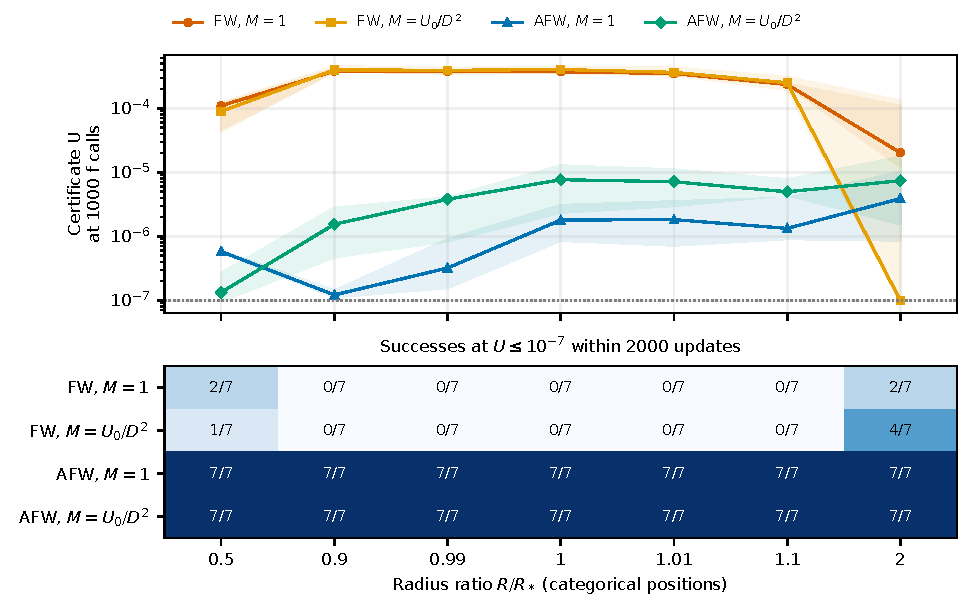
\includegraphics[width=\textwidth]{figures/constraint_transition.pdf}
\caption{Poisson activity sweep with equal weights on seven distinct
starts per radius. Top: median and interquartile certificate at 1000
function calls; completed runs are carried forward, and nonterminal
runs reach this budget. Bottom: successes at $10^{-7}$ within 2000
updates. Radius ratios occupy categorical positions, so their spacing
does not represent Euclidean distance. This is one dataset.}
\label{fig:transition}
\end{figure}
